\documentclass[12pt, a4paper] {ncc}
\usepackage[utf8] {inputenc}
\usepackage[T2A]{fontenc}
\usepackage[english, russian] {babel}
\usepackage[usenames,dvipsnames]{xcolor}
\usepackage{listings,a4wide,longtable,amsmath,amsfonts,graphicx,tikz}
\usepackage{pgfplots}
\usepackage{indentfirst}
\usepackage{bytefield}
\usepackage{multirow}
\usepackage{tabularx}

\begin{document}
\frenchspacing
\pagestyle{empty}
\begin{center}
     Национальный исследовательский университет информационных технологий,
                              механики и оптики\\
                        Кафедра вычислительной техники\\
                          Сети ЭВМ и телекоммуникации
\end{center}
\vspace{\stretch{2}}
\begin{center}
                            Домашняя работа №1\\
                <<Кодирование данных в телекоммуникационных сетях>>
\end{center}
\vspace{\stretch{3}}
\begin{flushright}
                                          Студентка:\\
                                                         {\it Куклина М., P3301}
\end{flushright}
\vspace{\stretch{4}}
\begin{center}
                             Санкт-Петербург, 2017
\end{center}
\newpage


\section{Цели работы}
	Изучение методов логического и физического кодирования, используемых в цифоровых сетях передачи данных.

\section{Формирование сообщений}
\begin{enumerate}
        \item Фамилия студента: \textsl{КУКЛИНА М.Д.};
        \item Представление в HEX: \texttt{CA D3 CA CB C8 CD C0 20 CC 2E C4 2E};
        \item Представление в BIN: \texttt{ 11001010 11010011 11001010 11001011
											   11001000 11001101 11000000 00100000
											   11001100 00101110 11000100 00101110
											 }
        \item Длина сообщения: \texttt{12 байт (96бит)}.
		\item Пропускная способность: 10 Мбит/с.
		\item Длительность битового интервала: $t_b = 100$ нс.
\end{enumerate}

\section*{Физическое кодирование}
	\subsection*{Манчестерское кодирование}
		\begin{figure}[h!]
			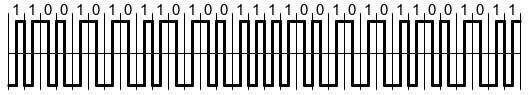
\includegraphics{../img/Manchester.png}
		\end{figure}
		\begin{enumerate}
			\item Частота основной гармоники: $f_0 = \frac {1} {t_b} = 10$ МГц 
			\item Нижняя граница частот: $f_l = \frac {1} {2t_b} = 5$ Мгц
			\item Верхняя граница частот: $f_h = 7f_0 = 70$ МГц
			\item Полоса пропускания: $f_h - f_l = 70 - 5 = 65$ МГц 
			\item Среднее значение частоты: $f_{avg} = 30$ \\
				  (для первых четырёх байт: $f_{avg} = \frac {4} {64} (24*f_0 + \frac {20 \cdot 2} {2} f_0) = 27.5 $)
		\end{enumerate}
	\subsection*{NRZ}
		\begin{figure}[h!]
			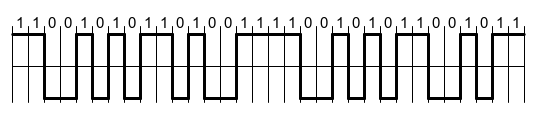
\includegraphics{../img/NRZ.png}
		\end{figure}
		\begin{enumerate}
			\item Частота основной гармоники: $f_0 = \frac {1} {2C} = 5$ Мгц
			\item Нижняя граница частот: $f_l = \frac {1} {16t_b} = 0.625$ МГц
			\item Верхняя граница частот: $f_h = 7f_0 = 35$ МГц 
 			\item Полоса пропускания: $f_h - f_l = 35 - 0.625 = 34.625$ МГц 
			\item Среднее значение частоты: $f_{avg} = 10$ \\
				  (для первых четырёх байт: $f_{avg} = \frac {4} {32} (12f_0 + \frac {16} {2} f_0 + \frac {4} {4} f_0) = 13.750$)
		\end{enumerate}
	\subsection*{RZ}
		\begin{figure}[h!]
			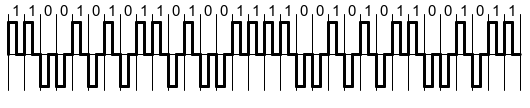
\includegraphics{../img/RZ.png}
		\end{figure}
		\begin{enumerate}
			\item Частота основной гармоники: $f_0 = \frac {1} {t_b} = 10$ МГц
			\item Нижняя граница частот: $f_l = \frac {1} {2t_b}= 5$ МГц
			\item Верхняя граница частот: $f_h = 7f_0 = 70$ МГц
			\item Полоса пропускания: $f_h - f_l = 70 - 5 = 65$ МГц
			\item Среднее значение частоты: $30$ МГц
					(для первых четырёх байт: $f_cp = 27.5$)
		\end{enumerate}
\section*{Сравнительный анализ методов физического кодирования}
    \begin{table}[!h]
        \begin{tabular}{|c|c|c|c|c|c|}
            \hline
                & $f_0$ & $f_l$, МГц & $f_h$, МГц & $F$, МГц & $f_{avg}$, МГц \\ \hline
            M   & 10    & 5          & 70         & 65       &  30      \\ \hline
            NRZ & 5     & 0.625      & 35         & 34.625   &  10       \\ \hline
            RZ  & 10    & 5          & 70         & 65       &  30      \\ \hline
        \end{tabular}
    \end{table}

    \begin{table}[!h]
        \begin{tabular}{|c|c|c|c|c|c|}
            \hline
                                                &  M  & NRZ & RZ \\ \hline
            Минимизация спектра                 &  -  & +   & -  \\ \hline
            Постоянная составляющая             &  -  & +   & -  \\ \hline
            Самосинхронизация                   &  +  & -   & +  \\ \hline
            Обнаружение ошибок и их исправление &  +  & -   & +  \\ \hline
            Низкая стоимость реализации         &  +  & +   & -  \\ \hline
        \end{tabular}
    \end{table}


	В качестве лучшего способа кодирования мною были выбраны манчестерское кодирование и метод
	кодирования NRZ. Первый их них обеспечивает самосинхронизацию, обнаружение и исправление ошибок
	на фоне низкой стоимости реализации кодирования и отсутсвия постоянной составляющей. Второй же  
	метод, не обладая самосинхронизацией (в исходном сообщении встречаются длинные последовательности
	нулей и единиц), имеет более высокую минимизацию спектра в сравнении с RZ и более
	низкую стоимость.

\section*{Логическое кодирование}
	\subsection*{4B/5B}
    	\begin{enumerate}
            \item Фамилия студента: \textsl{КУКЛИНА М.Д.};
            \item Представление в HEX: \texttt{ D5 B7 5D 5B 57 D4 B5 BD 7A 9E D6 A9 CD 2A 9C} ;
            \item Представление в BIN: \texttt{ 11010101 10110111 01011101 01011011 01010111 11010100 10110101 10111101 01111010 10011110 11010110 10101001 11001101 00101010 10011100}
            \item Длина сообщения: \texttt{12 байт (120 бит)}.
			\item Избыточность: 25 \% 
    		\item Пропускная способность: 10 Мбит/с.
    		\item Длительность битового интервала: $t_b = 100$ нс.
        \end{enumerate}	
	\subsection*{Манчестерское кодирование}
		\begin{figure}[h!]
			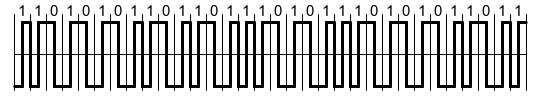
\includegraphics{../img/ManchesterLog.png}
		\end{figure}
		\begin{enumerate}
			\item Частота основной гармоники: $f_0 = \frac {1} {t_b} = 10$ МГц 
			\item Нижняя граница частот: $f_l = \frac {1} {2t_b} = 5$ Мгц
			\item Верхняя граница частот: $f_h = 7f_0 = 70$ МГц
			\item Полоса пропускания: $f_h - f_l = 70 - 5 = 65$ МГц 
			\item Среднее значение частоты: $f_{avg} = 26.333$ \\
				  (для первых четырёх байт: $f_{avg} = \frac {4} {64} (20*f_0 + \frac {22 \cdot 2} {2} f_0) = 26.25 $)
		\end{enumerate}
	\subsection*{NRZ}
		\begin{figure}[h!]
			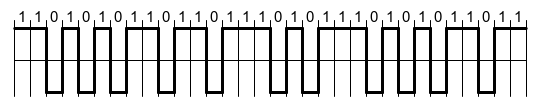
\includegraphics{../img/NRZLog.png}
		\end{figure}
		\begin{enumerate}
			\item Частота основной гармоники: $f_0 = \frac {1} {2C} = 5$ Мгц
			 \item Нижняя граница частот: $f_l = \frac {1} {5t_b} = 1$ МГц
			\item Верхняя граница частот: $f_h = 7f_0 = 35$ МГц 
 			\item Полоса пропускания: $f_h - f_l = 34$ МГц 
			\item Среднее значение частоты: $f_{avg} = 13.667$ \\
				  (для первых четырёх байт: $f_{avg} = \frac {4} {32} (16f_0 + \frac {5 \cdot 2} {2} f_0 + \frac {3 \cdot 2} {3} f_0) = 14.375$)
		\end{enumerate}
	\subsection*{Сравнительный анализ}
    \begin{table}[!h]
        \begin{tabular}{|c|c|c|c|c|c|}
            \hline
                & $f_0$ & $f_l$, МГц & $f_h$, МГц & $F$, МГц & $f_{avg}$, МГц \\ \hline
            M   & 10    & 5          & 70         & 65       &  26.333        \\ \hline
            NRZ & 5     & 1          & 35         & 34       &  13.667        \\ \hline
        \end{tabular}
    \end{table}

	Метод кодирования 4B/5B обеспечивает самосинхронизацию кодов (что можно наблюдать на последовательности
	закодированного сообщение методом NRZ, где ранее наличествующие длинные последовательности нулей и единиц
	исчезли) и возможность обнаружения ошибок. На фоне данных свойств ряд недостатков метода NRZ
	уменьшают вес, однако ряд достоинств манчестерского кода преумножаются в цене (к примеру, дополнительная защита от ошибок),
	вследствие чего манчестерский код лучший для передачи избыточного сообщения.

\section*{Скремблирование}

	Алгоритм скремблирования: $B_i = A_i \oplus B_{i-5} \oplus B_{i-7}$
	Исходное сообщение:  \texttt{ 11001010 11010011 11001010 11001011
        						  11001000 11001101 11000000 00100000
        						  11001100 00101110 11000100 00101110
						  }

	
	Скремблированное сообщение (BIN): \texttt { 11001101 00100000 10001111 10101001 
											   11010101 11001000 00010000 10000101
											   11101000 10111010 01100011 11110110
									  }
	Скремблированное сообщение (HEX): \texttt { CD 20 8F A9 D5 C8 10 85 E8 BA 63 F6 }

	Можно отметить отсутствие в полученном сообщении последовательности из 8-и нулей.

	\subsection*{Манчестерское кодирование}
		\begin{figure}[h!]
			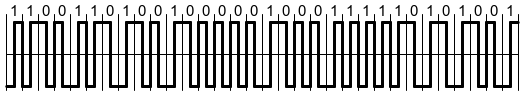
\includegraphics{../img/ManchesterS57.png}
		\end{figure}
		\begin{enumerate}
			\item Частота основной гармоники: $f_0 = \frac {1} {t_b} = 10$ МГц 
			\item Нижняя граница частот: $f_l = \frac {1} {12t_b} = 5$ Мгц
			\item Верхняя граница частот: $f_h = 7f_0 = 70$ МГц
			\item Полоса пропускания: $f_h - f_l = 70 - 5 = 65$ МГц 
			\item Среднее значение частоты: $f_{avg} = 30$ \\
				  (для первых четырёх байт: $f_{avg} = \frac {4} {64} (32*f_0 + \frac {16 \cdot 2} {2} f_0) = 30 $)
		\end{enumerate}
	\subsection*{NRZ}
		\begin{figure}[h!]
			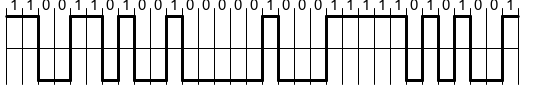
\includegraphics{../img/NRZS57.png}
		\end{figure}
		\begin{enumerate}
			\item Частота основной гармоники: $f_0 = \frac {1} {2C} = 5$ Мгц
			 \item Нижняя граница частот: $f_l = \frac {1} {6t_b} = 0.8333$ МГц
			\item Верхняя граница частот: $f_h = 7f_0 = 35$ МГц 
 			\item Полоса пропускания: $f_h - f_l = 34.167$ МГц 
			\item Среднее значение частоты: $f_{avg} = 10$ \\
				  (для первых четырёх байт: $f_{avg} = \frac {4} {32} (9f_0 + \frac {5 \cdot 2} {2} f_0 + \frac {3} {3} f_0 + \frac {5 \cdot 2} {5}) = 10.625$)
		\end{enumerate}


	\subsection*{Сравнительный анализ}
    \begin{table}[!h]
        \begin{tabular}{|c|c|c|c|c|c|}
            \hline
                & $f_0$ & $f_l$, МГц & $f_h$, МГц & $F$, МГц & $f_{avg}$, МГц \\ \hline
            M   & 10    & 5          & 70         & 65       &  30			  \\ \hline
            NRZ & 5     & 0.8333     & 35         & 34.167   &  10        \\ \hline
        \end{tabular}
    \end{table}
	
	Если сравнивать полученные данные с данными, полученными в первом пунтке, то можно заметить
	сужение пропускной способности для NRZ, пусть и незначительное; полученный код
	содержит меньшее количество последовательных нулей и единиц, что уменьшает вероятность
	рассинхронизации источника и проёмника, однако он всё ещё уступает манчестерскому кодированию,
    показатели которого не изменились, что говорит о том, что сравнительно лучше NRZ
    с точки зрения затрат на скремблирование. 

\section*{Вывод}

	В ходе выполнения домашней работы были изучены методы физического и логического кодирования.
	При передаче исходного сообщения без дополнительных операций над ним лучшие результаты показал
	манчестерский метод кодирования в сравнении с NRZ и RZ и в виду собственных представлений о
	полезности свойств (самосинхронизация, отсутствие постоянной составляющей, цена). 
	При анализе методов при избыточном и скремблированном сообщении было обнаружено, что манчестерский
	метод даёт лучшие характеристики (исключая ширину полосы пропускания) в сравнении с прочими
    рассмотренными. 
\end{document}
